\documentclass[10pt]{article}
\usepackage[margin=0.5in]{geometry}
\usepackage{tikz}
\usetikzlibrary{shapes.geometric, arrows.meta}

% Define custom styles for consistency and reuse
\tikzset{
  % The 'outline' style defines a 1.5pt thick black line for the shape border
  outline/.style={draw=black, line width=1.5pt},
  % The 'filled' style makes the shape interior solid black
  filled/.style={fill=black},
  % The 'leaf' style combines 'filled' and 'outline' for a leaf-like appearance
  leaf/.style={filled, outline, shape=regular polygon, regular polygon sides=4, minimum size=0.5cm},
  % The 'petal-outer' style is for the outer part of a petal, solid white with the black outline
  petal-outer/.style={fill=white, outline, shape=ellipse},
  % The 'petal-inner' style defines the spiral core, with a slightly thinner line
  petal-inner/.style={draw=black, line width=0.8pt},
  % The 'logo-text' style is for the main logo text
  logo-text/.style={font=\bfseries\Huge, anchor=center, text=black, inner sep=0pt},
  % The 'catchline-text' style is for the secondary text line
  catchline-text/.style={font=\large, anchor=center, text=black, inner sep=0pt}
}

\begin{document}
\pagestyle{empty}
\begin{center}
% The tikzpicture environment is used to create the drawing
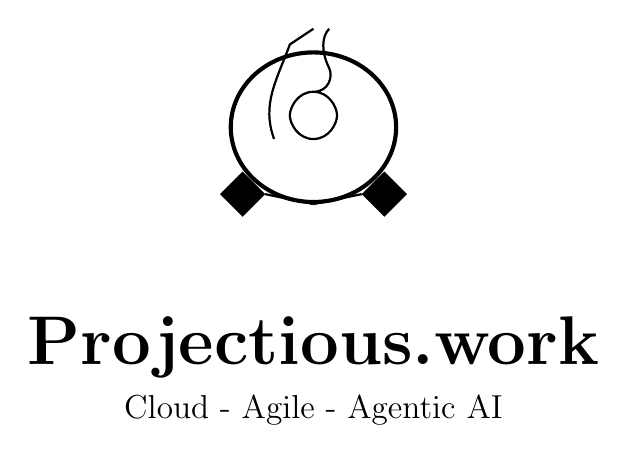
\begin{tikzpicture}

  % Draw the leaves at the bottom
  \node[leaf, xshift=-0.9cm, yshift=1.45cm, rotate=45] at (0,0) (left-leaf) {}; % Left leaf
  \node[leaf, xshift=0.9cm, yshift=1.45cm, rotate=-45] at (0,0) (right-leaf) {}; % Right leaf

  % Draw the outer flower bud structure
  \begin{scope}[yshift=1.45cm] % Group to apply shift to all contained shapes
    \node[petal-outer, minimum width=2.1cm, minimum height=1.9cm] at (0,0.85) (outer-bud) {};
  \end{scope}

  % Draw the inner spiral and lines, defining the core of the bud
  \begin{scope}[yshift=1.45cm, petal-inner] % Apply style to this scope
    % Outer petal lines to define the overall shape
    \draw (left-leaf.corner 4) -- (outer-bud.south);
    \draw (right-leaf.corner 3) -- (outer-bud.south);
    
    % Main line following the bud's contour
    \draw (-0.5,0.7) to[out=110, in=-110] (-0.3,1.9) -- (0,2.1);
    
    % Core spiral, drawn as a Bézier curve
    \draw (0,1.3) .. controls (0.2,1.3) and (0.3,1.1) .. (0.3,1.0) 
                  .. controls (0.3,0.9) and (0.2,0.7) .. (0,0.7)
                  .. controls (-0.2,0.7) and (-0.3,0.9) .. (-0.3,1.0)
                  .. controls (-0.3,1.1) and (-0.2,1.3) .. (0,1.3)
                  % Continuing with petal lines from the spiral core
                  .. controls (0.2,1.3) and (0.25,1.5) .. (0.2,1.6)
                  .. controls (0.1,1.8) and (0.1,2.0) .. (0.2,2.1);
  \end{scope}

  % Add the main text below the logo
  \node[logo-text] at (0,-0.5) (name) {Projectious.work};

  % Add the secondary catchline text below the main name
  \node[catchline-text] at (0,-1.3) {Cloud - Agile - Agentic AI};

\end{tikzpicture}
\end{center}
\end{document}
